\newpage
\chapter{Результати експериментів}

\section{Дослідження індикатрис розсіювання органо-неорганічних  гібридів pHEMA-TiO$_2$}
Одним із методів дослідження впливу наночастинок діоксиду титану оптичні властивості матеріалів є вимірювання кутового розподілу інтенсивності розсіяного світла (індикатриси розсіювання).
Експериментальнi данi розсiяння для слабкорозсiюючих зразкiв знаходяться в
межах широкого динамiчного дiапазону (близько 6-7 порядкiв величини сигналу).

В iзотропних середовищах розсiяння є аксiально-симетричним. Тому для
отримання iндикатриси зразка достатньо вимiряти кутовий розподiл потужності чи
iнтенсивностi випромінювання у будь-якiй площинi розсiяння (Рис. \ref{fig:ind1}).
Експериментальна лазерна установка для оптичної дiагностики зразкiв побудована на основi гонiометра
Г-5 з рiзними джерелами лазерного випромiнювання на його нерухомому плечi: DPSS діодним лазером (твердотільний
лазер з діодною накачкою, $\lambda = 532$ нм, потужнiсть випромiнювання P = 50 мВт) або
He-Ne лазером ($\lambda = 633$ нм, P = 10 мВт). Дослiджуваний зразок розмiщувався на
предметному столику, схему реєстрацiї було розташовано на рухомому плечi
гонiометра на вiдстанi L = 210 мм від зразка. Система реєстрацiї складалась з
астрономічної матриці .
%TODO  знайти інфу про матрицю

Дана експериментальна установка призначена для дослiдження полярної
кутової залежностi iнтенсивностi розсiяного зразком свiтла (по вiдношенню до
початкового напрямку поширення лазерного променя). Значення потужностi
випромiнювання у напрямку $\theta$ отримують пiдсумовуванням даних з усiх пiкселiв
детектора.

Кутовий розподiл розсiяного свiтла було вивчено при довжині хвилі 532 нм.
Вимiрювання проводилося в переднiй напiвсферi, тобто в кутовому дiапазонi
$0 \leq \theta \leq 90^o$.



\begin{figure}
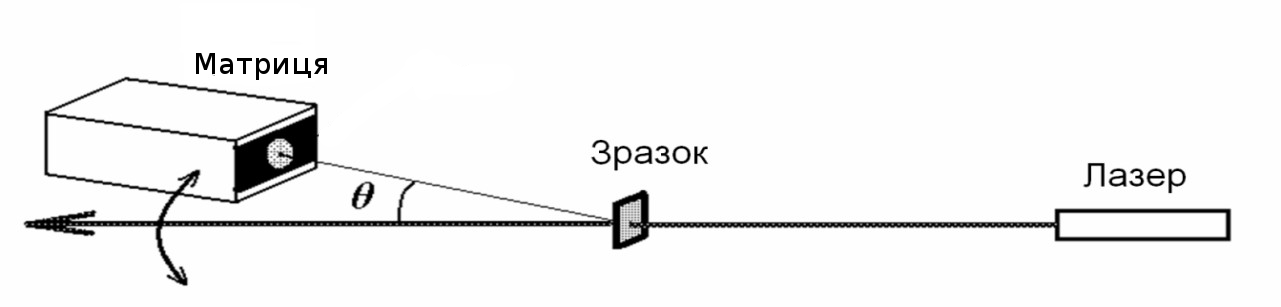
\includegraphics[width=16cm]{ind1}
\caption{Схема дослідження індикатриси розсіяння}\label{fig:ind1}

\end{figure}


Індикатриси розсіянн на довжині хвилі 532 нм для гібридів з різною концентрацією TiO$_2$ зображено на Рис. \ref{fig:ind2}.

\begin{figure}
\centering
\includegraphics[width=16cm]{./graph/Indic/plot}
\caption{Індикатриси розсіяння на довжині хвилі 532 нм для різних концентрацій інкорпорованих наночастинок TiO$_2$}\label{fig:ind2}
\end{figure}

Дані на індикатрисах подано у напівлогарифмічному масштабі по осі ординат для того, щоб
підкреслити великий динамічний діапазон даного процесу -- величина сигналу
змінюється приблизно на 6-7 порядків під час переходу від напрямку, що відповідає
поширенню лазерного пучка, до великих кутів розсіяння.

Зобразивши дані в подвійному логарифмічному масштабі, можна більш детально описати фізичне походження кожної з частин діапазону (Рис. \ref{fig:ind3}). В такій інтерпретації даних чітко видно три діапазони, що відповідають різним етапам експерименту:
\begin{enumerate}[I]
\item $\theta<1^o$ -- "плато"; 
\item $1^o<\theta<2^o$ -- "обрив";
\item $\theta>2^o$ -- "крила" індикатриси.
\end{enumerate}


Перший діапазон (I) характеризується найбiльшим
спотворенням вхiдних даних, оскільки майже все лазерне випромінювання, що пройшло через зразок, потраплає на детектор(геометрiя реєстрацiї балiстичних фотонiв). Внаслiдок цього отриманi данi не залежать вiд кутового положення детектора.

У другому діапазоні (II) спостерігається різке зниження сигналу, що відповідає етапу виходу детектора з області прямого поширення променя і переходу в область геометричної тіні. Ця область характеризується значними похибками, що викликані неточністю кутового позиціонування реєструючого пристрою. 

В третьому діапазоні детектор збирає лише випромінювання, що розсіялось зразком.В зразків, що досліджуються відсутні чіткі просторові структури, що підтверджується гладкістю кривої в логарифмічному масштабі. В діапазоні $2^o<\theta<30^o$ для всіх зразків спостерігається майже лінійна залежність з кутовим нахилом $-2.54 \pm 0.02$. Це означає, що розсiяна
потужнiсть випромiнювання розподiляється вздовж напрямку $\theta$ за оберненим
квадратичним законом $\Delta P(\theta) \approx \theta^{-2}$.

\begin{figure}
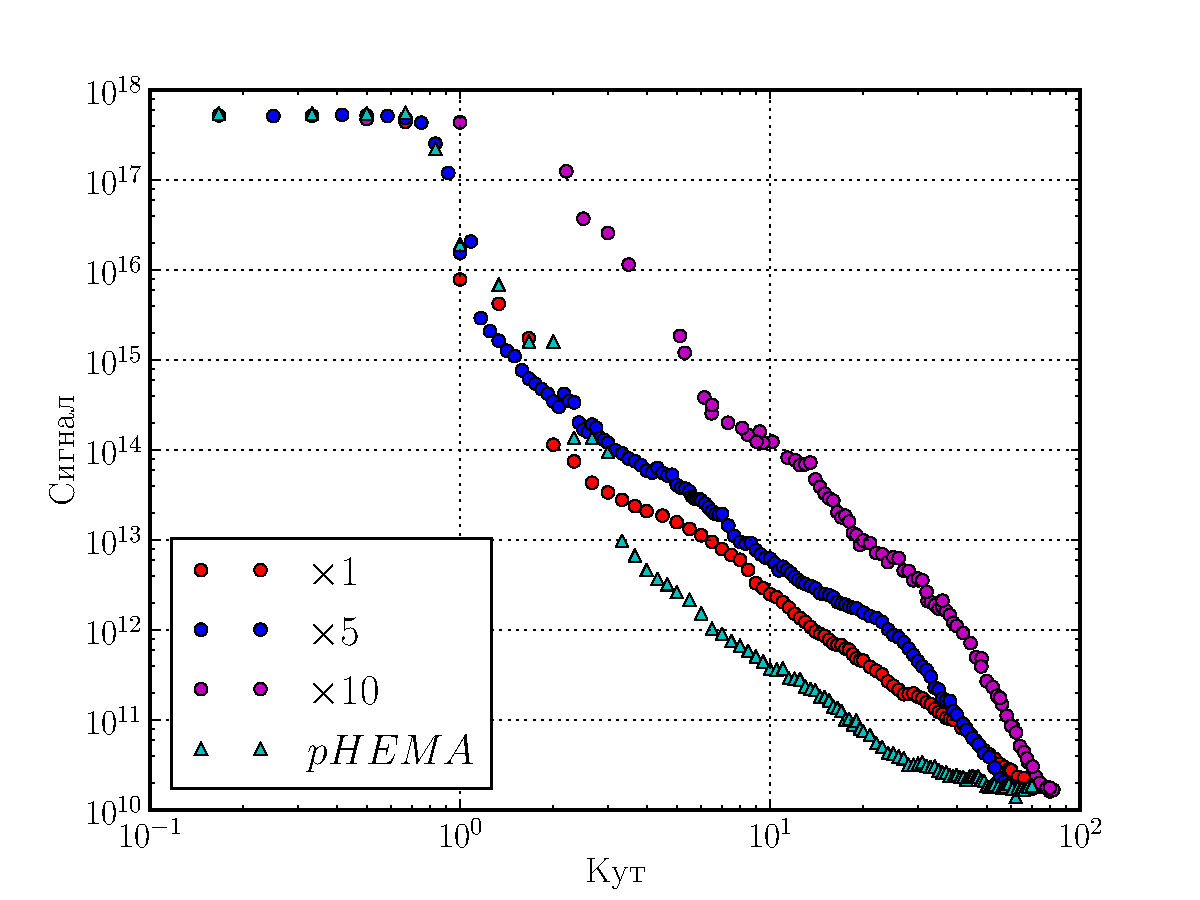
\includegraphics[width=16cm]{./graph/Indic/plot2}
\caption{Індикатриси розсіяння в подвійному логарифмічному масштабі для різних концентрацій інкорпорованих наночастинок TiO$_2$}\label{fig:ind3}
\end{figure}

Данi кутового розподiлу розсiяного випромiнювання у третьому дiапазонi
спотворюються дуже слабо, тому зареєстрована iндикатриса близька до реальної. Це
дає можливiсть обчислити втрати на розсiяння в переднiй напiвсферi всiх
дослiджуваних зразкiв. Метод обчислення ґрунтується на iнтегруваннi потужностi
розсiяного випромiнювання $\Delta P(\theta)$ в тiлесному кутi $\Delta \Omega$ по частинi передньої
напiвсфери, що вiдповiдає третiй дiлянцi на Рис. \ref{fig:ind3}:

\begin{equation}\label{eq:P_scat}
P_{scat} = \frac{2\pi}{P_0} \int_{\theta_{min}}^{\frac{\pi}{2}} \frac{\Delta P(\theta)}{\Delta \Omega} \sin{\theta} d\theta 
\end{equation}

Результати оцінки втрат на розсіяння для гібридних зразків з різними концентраціями TiO$_2$ наведено в таблиці \ref{tab:TabInd}

\begin{table}
\centering
\begin{tabular}{|c|c|c|}
\hline
Позначення & Концентрація TiO$_2$, мас. \% & \\ \hline

$pHEMA$		&	0		&	1.45 \\\hline
$\times1$	&	0,88	&	1.46 \\\hline
$\times5$	&	4,4		&	1.54\\\hline
$\times10$	&	8,8		&	7.3\\\hline
\end{tabular}
\caption{Втрати на розсіяння в передню на півсферу для зразків органо-неорганічних гібридів}\label{tab:TabInd}
\end{table}

З розрахунків видно, що із збільшенням концентрації інкорпорованих наночастинок TiO$_2$ розсіяння від зразків в передню напівсферу зростає. Зростання втрат на розсiяння при збiльшеннi концентрацiї наночастинок пояснюється виникненням ефекту самодефокусування при
збудженнi неперервним лазерним випромiнюванням iз довжиною хвилi 532 нм
внаслiдок резонансного збудження наночастинок анатазу. Цей ефект приводить до
пiдвищення оптичного контрасту в околi наночастинки i до збiльшення поперечного
розмiру розсiяння.


\section{Результати дослідження фотоіндукованих змін оптичного пропускання гібридів pHEMA-TiO$_2$}

Дослідження фотоіндукованих змін оптичного пропускання органо-неорганічних гібридів pHEMA-TiO$_2$
досліджувалися у геометрії повного пропускання (видозмінена схема Рис. \ref{fig:s1}).
Використовувався лазер Л1, схема та характеристики якого описані в пункті \ref{sec:L1}. Зразок ставився якомога ближче до фотодіода, відстань
від лінзи до зразка варіювалася в діапазоні 10-20 см, при фокусній відстані лінзи 8
см, для зміни радіусу лазерного пучка, що падає на зразок, а, відповідно і діапазону
інтенсивності, в якому проходить вимірювання при повному проході атенюатора.

На Рис. \ref{fig:TTrans} показані залежності повного пропускання від інтенсивності для
зразків з різною концентрацією TiO$_2$.

\begin{figure}
\centering
\includegraphics[width=16cm]{./graph/TTrans/plot}
\caption{Залежність повного пропускання зразків від падаючої
інтенсивності. pHEMA -- чистий гібридний зразок; концентрації для зразків $\times1 - \times20$ наведені в таблиці \ref{tab:Tab1}}\label{fig:TTrans}
\end{figure}

З рисунку видно, що, при збільшенні інтенсивності падаючого випромінювання, відбувається фотоіндуковане затемнення($\Delta T$) кожного із зразків. 
При цьому для зразків з малою концентрацією TiO$_2$ ($\times1, ~\times2,\times5$ ) за великих інтенсивностей характерне насичення. В цих зразках спостерігається незначне ($<1.5\%$) фотоіндуковане затемнення, як і в чистого зразка без TiO$_2$.

Зі збільшенням концентрації інкорпорованих частинок TiO$_2$ спостерігається зростання нелінійних ефектів. З рисунку \ref{fig:TTrans} видно різке зростання фотоіндукованого затемнення для зразків $\times10$ та $\times20$.

На основі отриманих залежностей повного пропускання від інтенсивності для зразків з різною концентрацією частинок TiO$_2$ було розраховано Уявну частину кубічної нелінійної сприйнятливості $Im(\chi^{(3)})$ для двох діапазонів інтенсивностей:
\begin{enumerate}
\item $0 < I <150 \frac{\textbf{МВт}}{cm^2}$ ("мала" інтенсивність);
\item $1250 < I <1500 \frac{\textbf{МВт}}{cm^2}$ ("велика" інтенсивність).
\end{enumerate}
Результати обрахунків занесено до таблиці \ref{tab:Tab1}. Графічну інтерпритацію цих даних зображено на рисунку \ref{fig:ImHi3}. На ній можна виділити групу зразків ($\times1 - \times5$) з малими концентраціями інкорпорованих частинок, для яких фотоіндуковані ефекти малі та майже не відрізняються від тих, що спостерігаються для чистого гібридного зразка pHEMA. Інша група зразків ($\times10, ~ \times20$) суттєво відрізняється від попередньої на обох діапазонах інтенсивностей.




\begin{figure}
\centering
\includegraphics[width=15cm]{./graph/ImHi3Gr/plot}
\caption{Залежність уявної частини нелінійної сприйнятливості третьго порядку $Im(\chi^{(3)})$ від концентрації частинок TiO$_2$}\label{fig:ImHi3}
\end{figure}

\begin{table}
\begin{tabular}{|>{\centering\arraybackslash}p{1.5cm}|>{\centering\arraybackslash}m{
3cm}|c|c|c|c|c|c|}
\hline
Ум. позн. & Концентрація TiO$_2$, \newline $\times 10^{20} ~ cm ^{-3}$ & \multicolumn{2}{c}{  $0 < I <150 \frac{\textbf{МВт}}{cm^2}$} & \multicolumn{2}{|c|}{$1250 < I <1500 \frac{\textbf{МВт}}{cm^2}$}\\
\cline{3-6}
 & & $Im(\chi)^{(3)},~ \times10^{-13}$ & $Re(\chi^{(3)}),~ \times10^{-11}$ & $Im(\chi^{(3)})$ & $Re(\chi^{(3)})$\\ 
\hline
$pHEMA$		&	0		&	9,37	&	-1,2	&	1.92	&	1,83	\\\hline
$\times1$	&	0,88	&	12,4	&	-10		&	0.757	&	1.37	\\\hline
$\times2$	&	1,76	&	9,47	&	-0,37	&	-0.85	&	-2.04	\\\hline
$\times5$	&	4,4		&	9,05	&	-4,2	&	0.98	&	1.32	\\\hline
$\times10$	&	8,8		&	10,4	&	-21		&	4.2		&	1.76	\\\hline
$\times20$	&	17,6	&	23,8	&	-21		&	2.28	&	2.71	\\\hline

\end{tabular}
\\[10pt]
\caption{Концентраційна залежність уявної $Im(\chi^{(3)})$ та дійсної $Re(\chi^{(3)})$  частин нелінійної сприйнятливості третього порядку. Величини наведені в одиницях СГС$_e$ }\label{tab:Tab1}
\end{table}


\section{Результати дослідження фотоіндукованих змін приосьового пропускання гібридів pHEMA-TiO$_2$}

Залежність приосьового пропускання від інтенсивності зразків органо-неоргінічних гібридів pHEMA-TiO$_2$ досліджувалась у схемі, що зображена на рис. \ref{fig:s1}. В даній схемі одночасно вимірюються зміни при приосьового пропускання зразка зі змінами приосьового пропускання в далекому полі. Використовувався лазер Л1 (рис. \ref{fig:las1}) з довжиною хвилі 1064 нм. 

На Рис. \ref{fig:OnAxDivTot} показані залежності приосьового пропускання від інтенсивності для гібридів pHEMA-TiO$_2$, віднормовані на припускання в далекому полі. З рисунку видно, що фотоіндуковані зміни приосьового пропускання суттєво залежать від зміни концентрації інкорпорованих частинок TiO$_2$ при збільшенні інтенсивності падаючого випромінювання.

Для зразків $\times1$, $\times5$ - $\times20$ та чистого pHEMA на початковому діапазоні інтенсивності ($<600~ \frac{\textbf{МВт}}{cm^2}$) спостерігається зменшення значення приосьового пропускання, що відповідає явищу самодефокусування ($\Delta n_{NLO} < 0$). При подальшому збільшенні інтенсивності ефект самодефокусування насичується та переходить в самофокусування. Для зразка $\times2$ ефект самодефокусування починає проявлятися лише при високій інтенсивності падаючого випромінювання ($I>1200 ~\frac{\textbf{МВт}}{cm^2}$). 
 
На основі отриманих залежностей осьового пропускання від інтенсивності для
зразків органо-неорганічних гібридів були обраховані значення дійсної частини кубічної нелінійної сприйнятливості $Re(\chi^{(3)})$ для двох діапазонів інтенсивностей:
\begin{enumerate}
\item $0 < I <150 \frac{\textbf{МВт}}{cm^2}$ ("мала" інтенсивність);
\item $1250 < I <1500 \frac{\textbf{МВт}}{cm^2}$ ("велика" інтенсивність).
\end{enumerate}
 
Результати обрахунків занесено до таблиці \ref{tab:Tab1} та зображено графічно на рис. \ref{fig:ReHi3}. Як і у випадку $Im(\chi^{(3)})$ можна виділити дві групи зразків з різними концентраціями TiO$_2$, зі схожими властивостями. Бачимо, що зміна концентрації інкорпорованих частинок TiO$_2$ суттєво впливає на величину нелінійних ефектів на різних діапазонах інтенсивності падаючого випромінювання. 
\begin{figure}
\centering
\includegraphics[width=16cm]{./graph/OnAxDivTotal/plot}
\caption{Залежність приосьового пропускання зразків від падаючої
інтенсивності.}\label{fig:OnAxDivTot}
\end{figure}


\begin{figure}
\centering
\includegraphics[width=15cm]{./graph/ReHi3Gr/plot}
\caption{Залежність дійсної частини нелінійної сприйнятливості третьго порядку $Re(\chi^{(3)})$ від концентрації частинок TiO$_2$}\label{fig:ReHi3}
\end{figure}

\section{Дослідження змін коефіцієнтів поглинання та заломлення}

The UV irradiation of pHEMA/TiO2-based hybrids materials induces modifications of
both absorption coefficient and refractive index. The total and on-axis transmittances, as a
function of the UV irradiation dose, are shown in Figs. 3(a) and 3(b) respectively. In the same
experimental conditions, the transmittance of the pure pHEMA reference sample is found
unaffected by the irradiation, which evidence that the effect is entirely due the presence of the
inorganic TiO2 component. 

In pHEMA/TiO2-based hybrids materials, the darkening is assigned to Ti+3 centers
which are formed by the CB electron trapping on Ti4+ after photoexcitation below 380 nm
( $h\nu \geq E_g = 3.2$ eV ). The scheme of the relevant processes involved in the Ti3+ centers
formation is drawn in the Fig. 4. The absorption of a photon $h\nu$ results in the electron
transition from the valence band, due to O2- 2p orbital, to the conduction band, due to Ti4+ 3d
orbital. Whereas the hole is supposed to escape rapidly into the organic pHEMA component,
the remaining CB electron is trapped into the inorganic component with the quantum
efficiency $\eta_a$ . The spontaneous relaxation of the photoinduced charges is slow resulting in a
Ti3+ centers lifetime of several weeks [10]. On the other hand, the maximal concentration of
the Ti3+ centers is limited by the inner-photoeffect, which corresponds to the trapped electrons
excitation. The successfully reexcited electrons can leave the inorganic component, and
recombine with holes localized in the organic component. This last process is characterized by
the quantum efficiency $\eta_b$ . 

Схема експерименту наведена на рис \ref{fig:s2}. Джерелом лазерного випромінювання виступав лізерний діод з довжиною хвилі випромінювання $\lambda = 375$ нм.

\begin{figure}
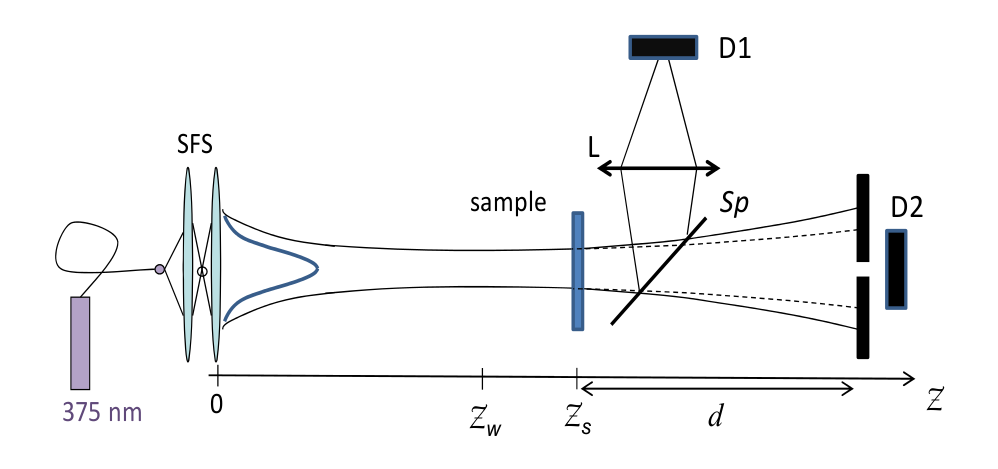
\includegraphics[width=16cm]{s2}
\caption{Схема експерименту для дослідження повного та приосьового пропускання на довжині хвилі $\lambda = 375$ нм. SFS -- система просторової фільтрації, Sp -- поділююча пластинка, S -- зразок, D1 і D2 -- фотодіоди}\label{fig:s2}
\end{figure}
\pagebreak
\begin{figure}
\centering
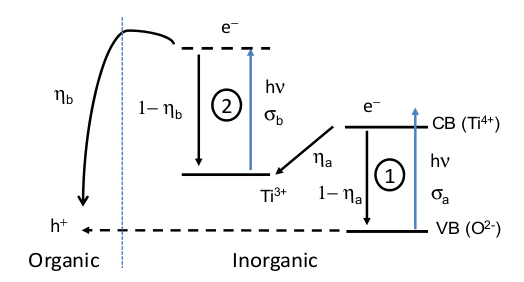
\includegraphics[width=12cm]{scheme}
\caption{Схема відповідних процесів, залучених в фотозатемненні pHEMA-TiO$_2$ гібридних матеріалів}\label{fig:s_pd}
\end{figure}

 The obtained quantum efficiencies $\eta_a$ for the
charge separation process are ranging from 13.5\% to 16.5\% excepted for the sample X5 for
which $\eta_a$ = 7\% . A less efficient polymerizatin in sample X5 may account for this difference.
The quantum efficiency $\eta_b$ of the inner photoeffect process is ranging from 1.5\% to 2.5\% for
all samples. The values of $\eta_a$ are reported in Table 1.

Графічна інтерпретація даних для квантового виходу та коефіцієнту поглинання зображена на Рис. \ref{fig:qa}.a) та \ref{fig:qa}.б). З рисунків видно, що результати даного експерименту корелюють з результатами дослідження повного та приосьового пропускання на довжині хвилі $\lambda=1064$ нм. В зображених концентраційних залежностях можна виділити дві групи зразків, як і в попередніх дослідах.

\begin{figure}
\begin{tabular}{c}

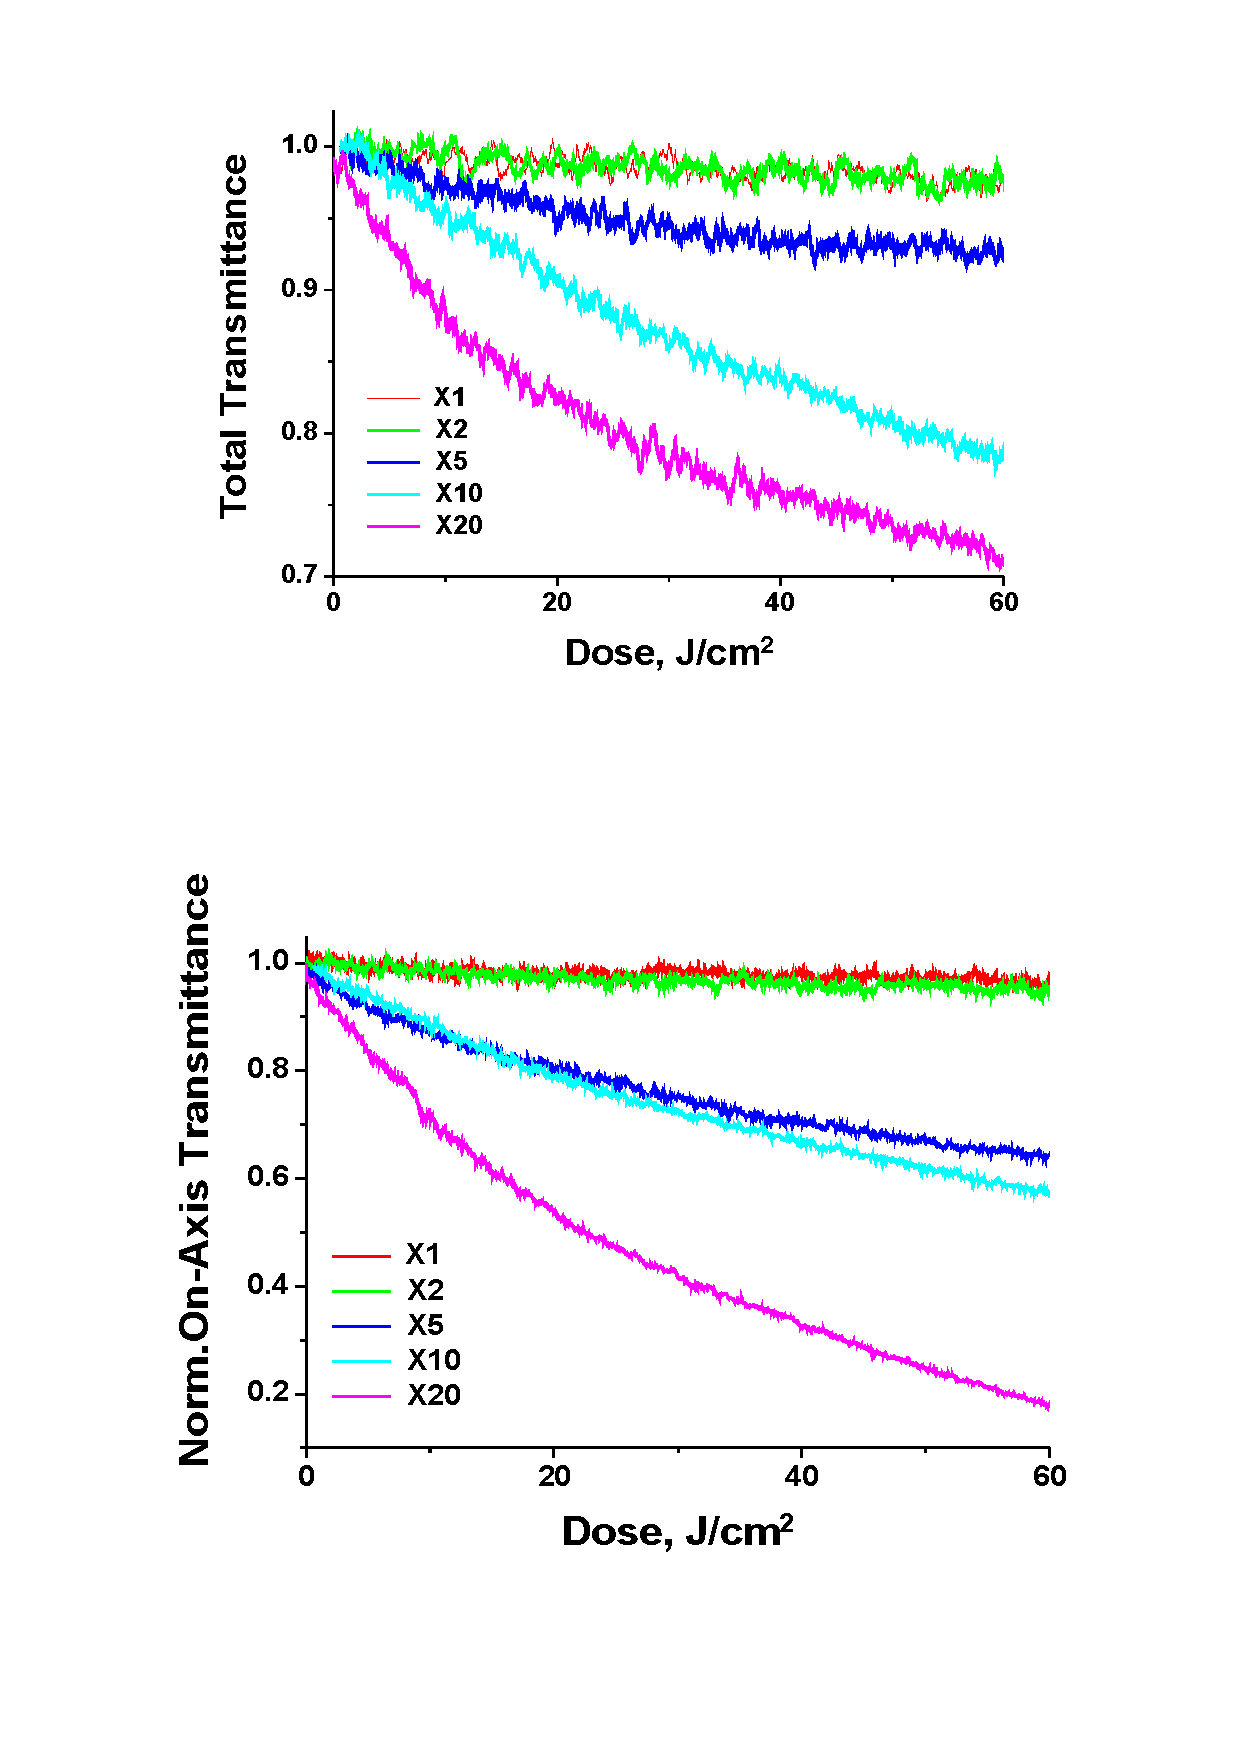
\includegraphics[clip=true, viewport=3cm 3cm 18cm 14cm, width=13cm ]{double1}
 \\
а)\\

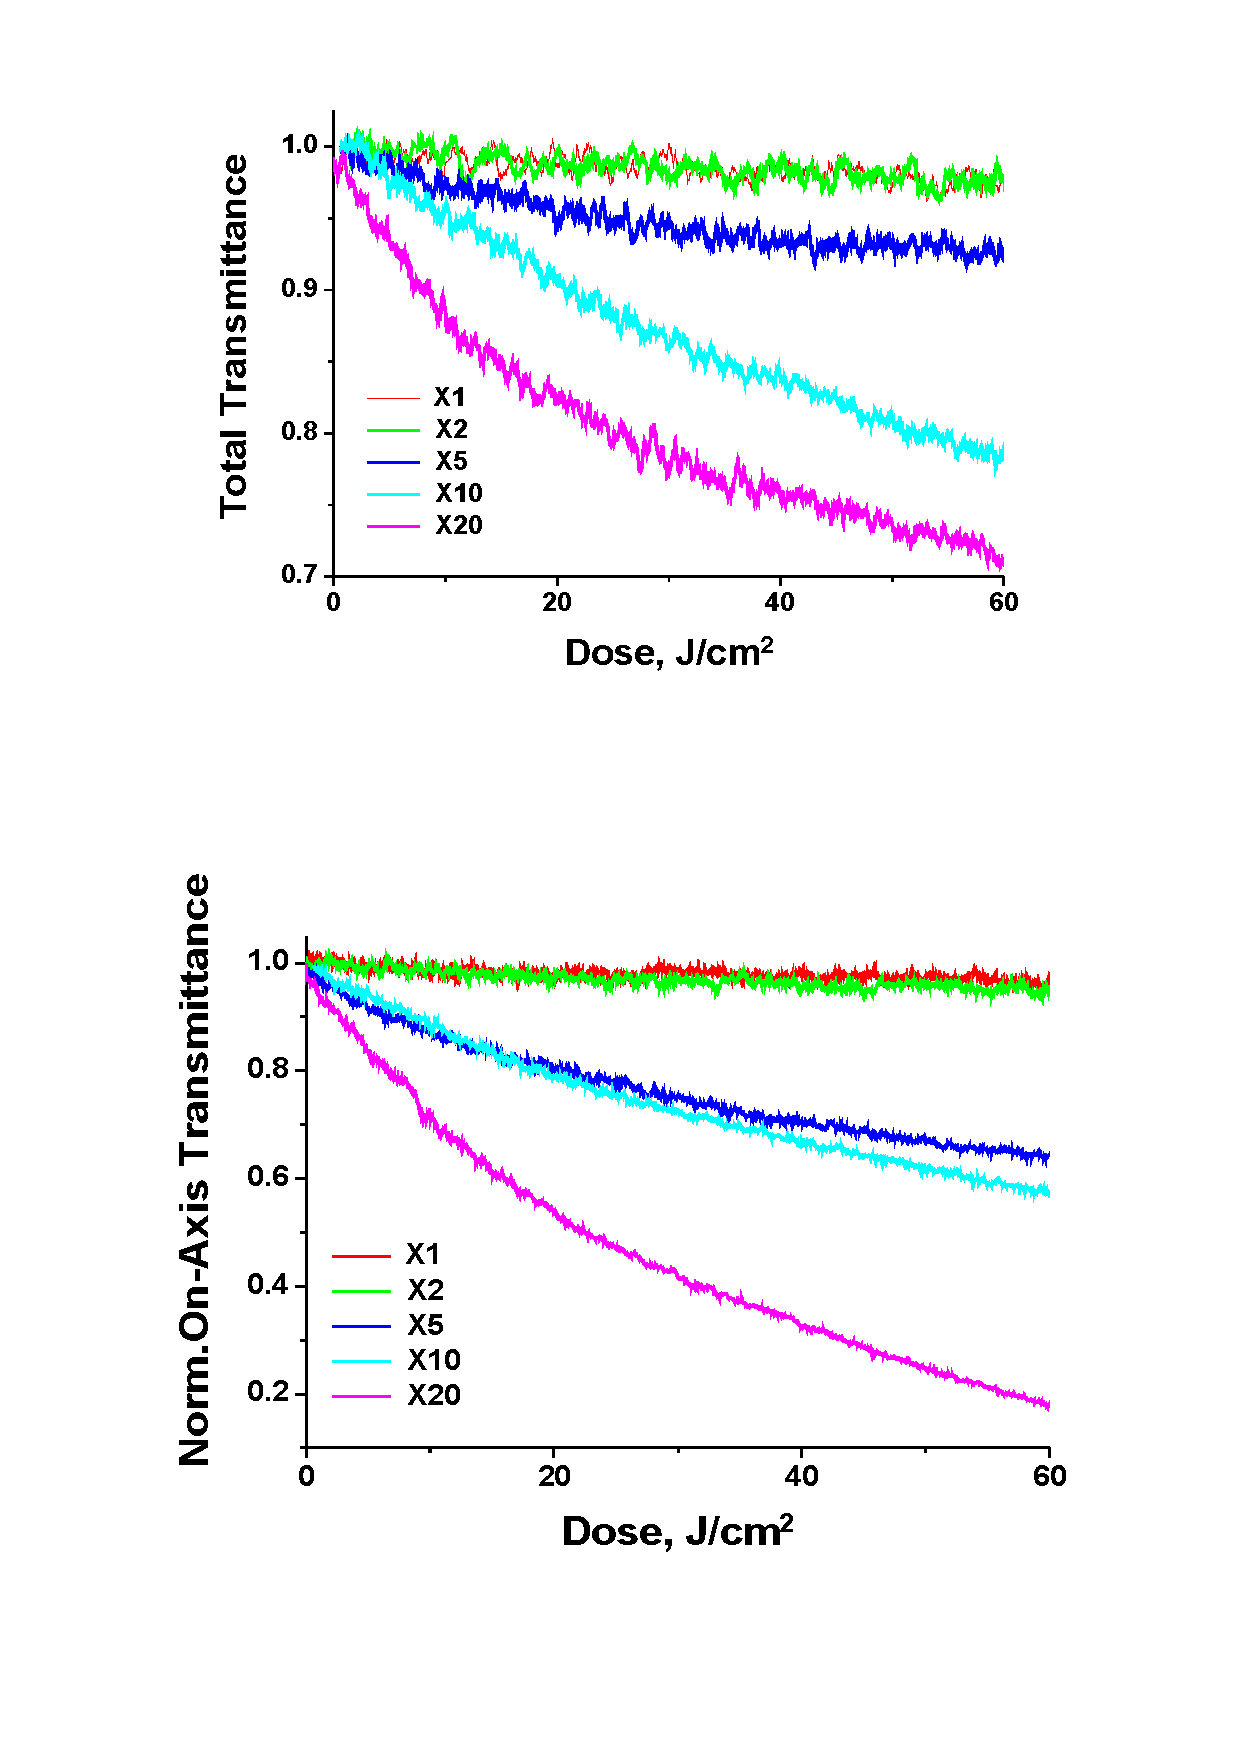
\includegraphics[clip=true, viewport=2cm 18cm 18cm 28cm ]{double1}
\\
б)
\end{tabular}
\caption{Зміна повного (a) та приосьового пропускання (б) і гібридних зразках як функція дози опромінення}\label{fig:dose}
\end{figure}


\begin{table}
\begin{tabularx}{\textwidth}{ |>{\centering}X|>{\centering}X|>{\centering}X|>{\centering}X|>{\centering}X|>{\centering}X|>{\centering}X|}
\hline

Зразок & $\Big[Ti^{4+}\Big]$ Конц, $\times 10^{20} cm^{-3}$ & Товщина (L), $\mu m$ & $\Delta n_0,\newline \times 10^{-4}$ & $\eta_a\newline @375 \text{нм}, \%$ & $\Big[ Ti^{3+} \Big] \newline {\times10 }^{17} ~ cm^{-3}$ & $a_0 = \frac{\Delta n_0}{\Big[ Ti^{3+} \Big] } \newline {\times10} ^{-22} ~ cm^{3}$  \tabularnewline
  \hline
$\times1$	&	0.88	&	94.9	&	-0.14	&	12.6	&	0.43	&	-0.33 \tabularnewline
  \hline
$\times2$	&	1.76	&	78.1	&	-0.42	&	12.6	&	0.86	&	-0.49  \tabularnewline
  \hline
$\times5$	&	4.40	&	104.4	&	-3.20	&	11.3	&	1.91	&	-1.68 \tabularnewline
  \hline
$\times10$	&	8.80	&	98.6	&	-6.40	&	16.5	&	6.05	&	-1.06  \tabularnewline
  \hline
$\times20$	&	17.6	&	82.7	&	-10.05	&	20.6	&	13.26	&	-0.76  \tabularnewline\hline
\end{tabularx}
\caption{Концентраційна залежність квантового виходу та коефіцієнту пропускання на довжині хвилі $\lambda=375$ нм}\label{tab:n_a-a}
\end{table}






\begin{figure}
\begin{tabular}{c}

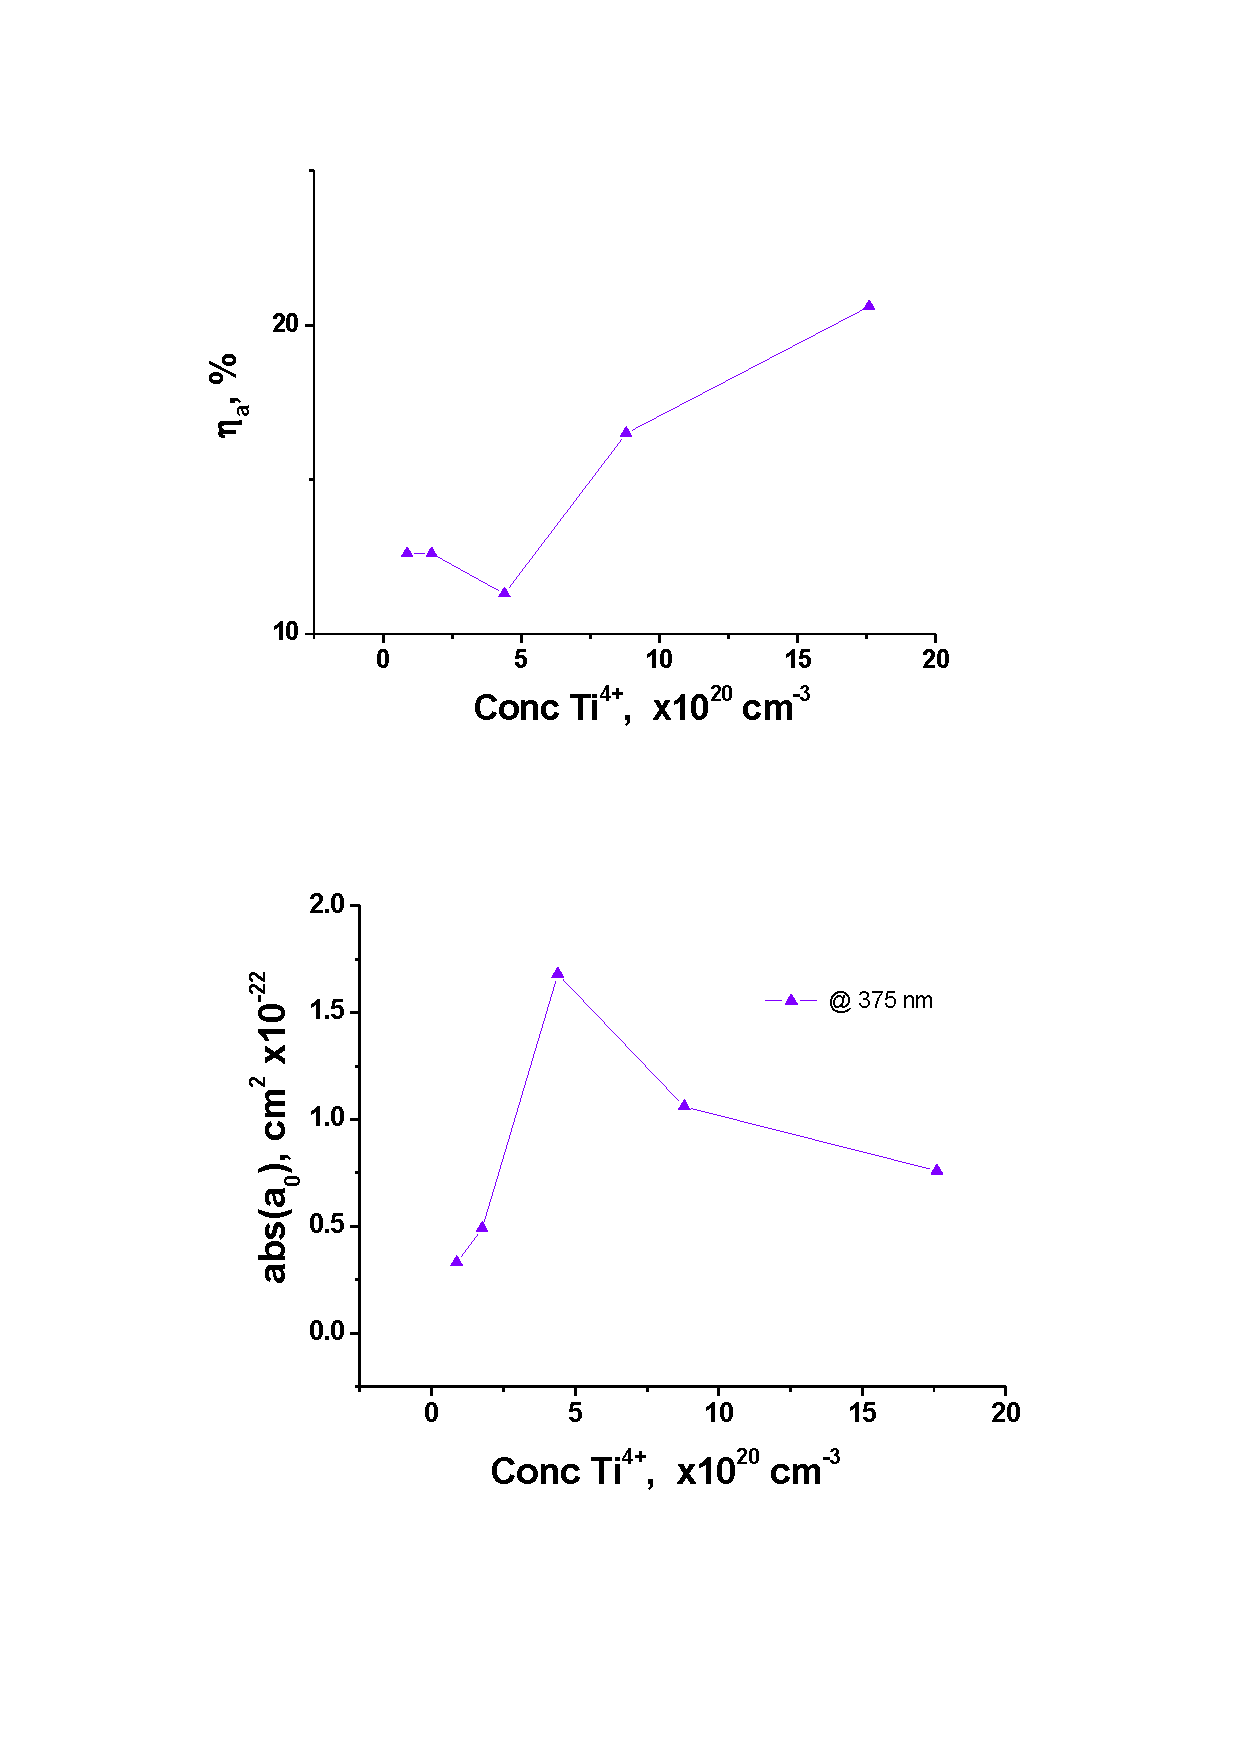
\includegraphics[clip=true, viewport=4cm 4cm 18cm 14cm ]{double2}\\
а)\\
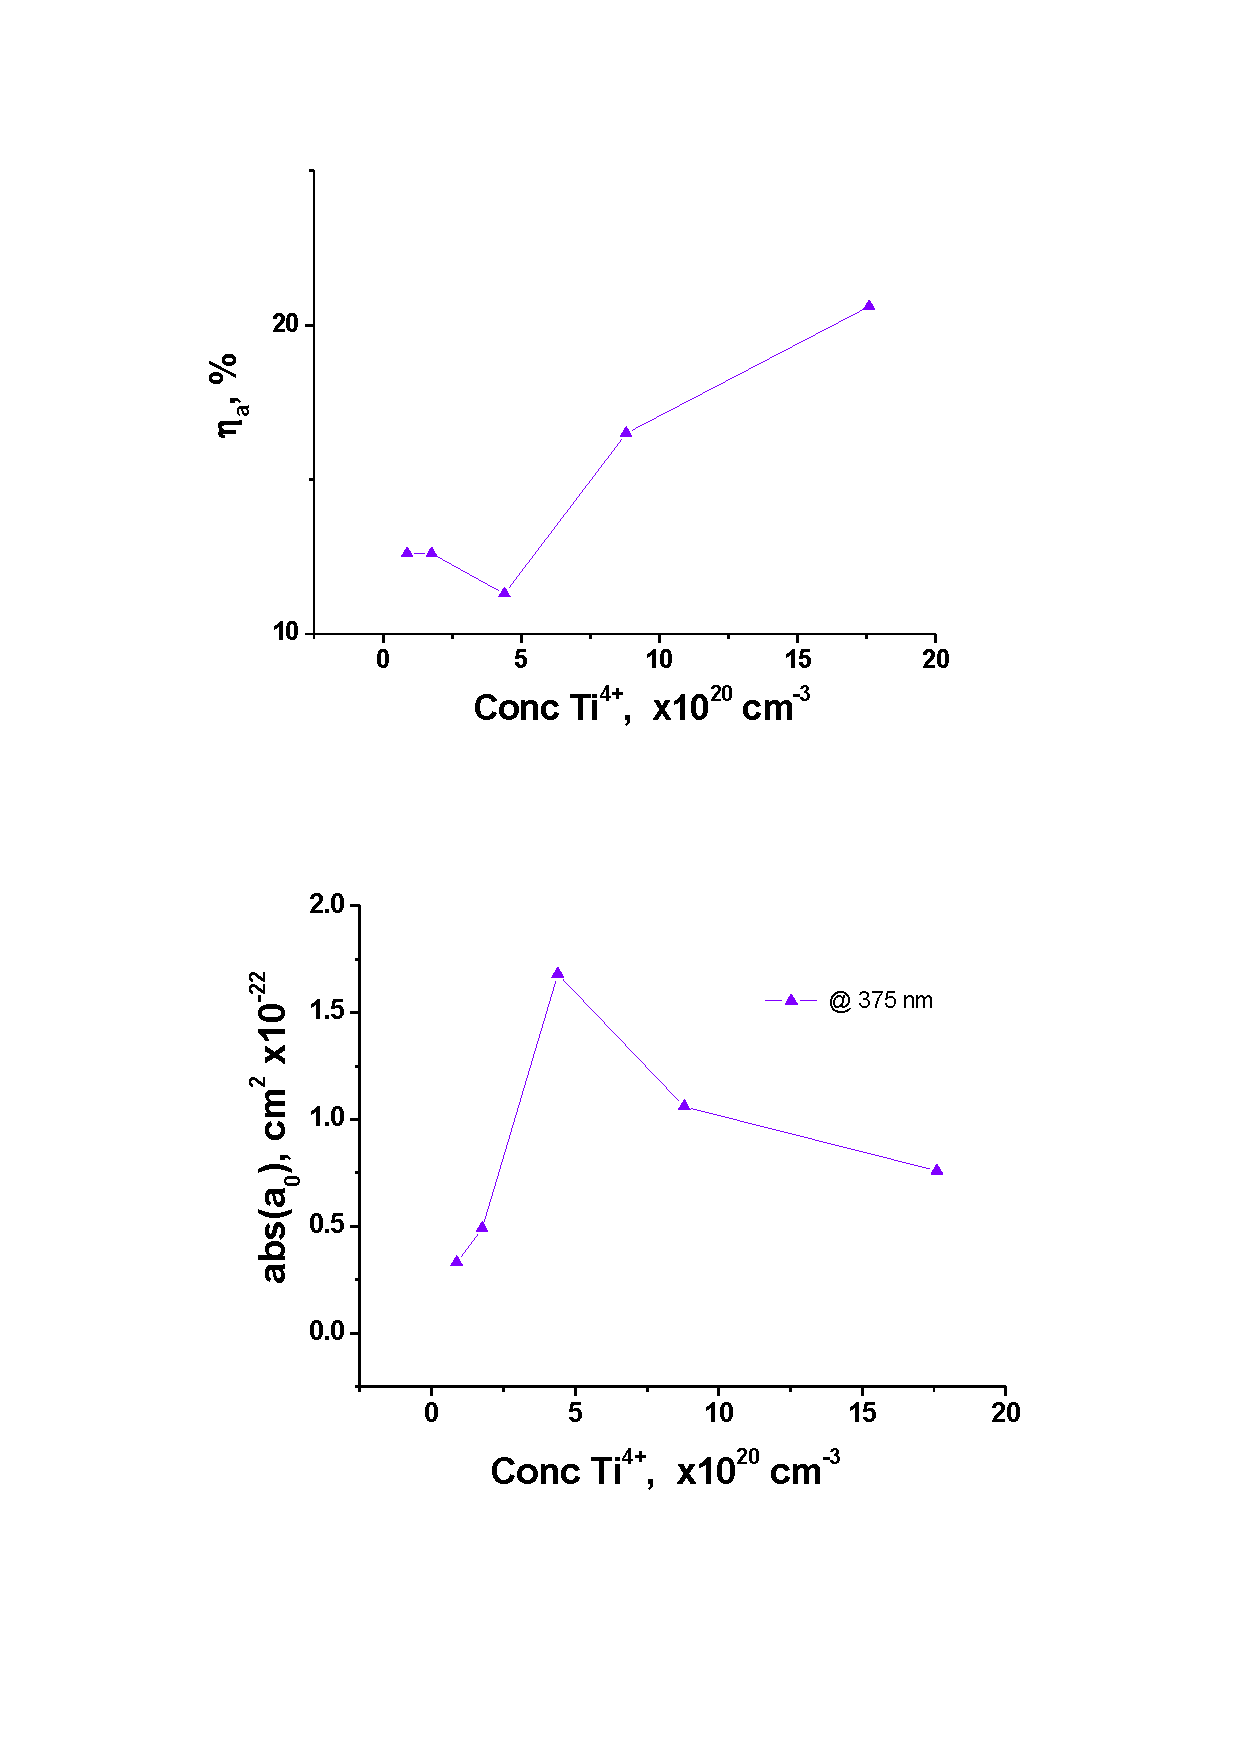
\includegraphics[clip=true, viewport=3cm 17cm 18cm 27cm ]{double2}
\\
б)
\end{tabular}
\caption{Залежність коефіцієнту поглинання (а) та квантового виходу (б)  від концентрації інкорпорованих частинок}\label{fig:qa}
\end{figure}
